\chapter{Έλεγχος}
\label{ch:testing}
Στο κεφάλαιο αυτό θα αναλυθούν οι έλεγχοι που υλοποιήθηκαν για τον κώδικα της εφαρμογής. 
Ο έλεγχος χωρίστηκε σε δύο επιμέρους κατηγορίες, στον έλεγχο του εργαλείου και στον έλεγχο των μοτίβων που υλοποιεί το εργαλείο.
Για την υλοποίησή τους χρησιμοποιήθηκε η βιβλιοθήκη Junit 4.
\section{Έλεγχος δομής σχεδιαστικών μοτίβων}
\label{sec:patternTesting}
\subsection{Έλεγχος μεθόδων φορτώματος μοτίβων}
\label{subsec:patternManagerTesting}
Σε αυτήν την ενότητα, θα παρουσιαστούν οι έλεγχοι για την δομή των μοτίβων τα οποία περιγράφονται στο αρχείο xml που δέχεται ως είσοδο 
το εργαλείο μας, Pattern Genius.
Για να επιβεβαιώσουμε την σωστή δομή κάθε μοτίβου, το μόνο που χρειάζεται είναι να ελέγξουμε την κλάση, η οποία δημιουργεί 
τα απαραίτητα αντικείμενα αντλώντας δεδομένα από το αρχείο περιγραφής των μοτίβων, η κλάση αυτή είναι η PatternManager.
Έχουμε δημιουργήσει τεστ τα οποία ελέγχουν εάν οι κλάσεις κάθε μοτίβου έχουν το σωστό όνομα, υλοποιούν ή επεκτείνουν την σωστή 
διεπαφή ή κλάση αντίστοιχα και περιέχουν τις σωστές μεθόδους και πεδία. Επίσης υπάρχουν τεστ τα οποία επιβεβαιώνουν την δομή των 
διεπαφών, ελέγχοντας το όνομα και τις μεθόδους κάθε διεπαφής. Οι περιπτώσεις ελέγχων χωρίστηκαν σε δύο πακέτα, 
στο ένα πακέτο υπάρχουν οι περιπτώσεις ελέγχου των κλάσεων κάθε μοτίβου και στο άλλο πακέτο υπάρχουν οι περιπτώσεις ελέγχου 
των διεπαφών κάθε μοτίβου. Πιο συγκεκριμένα, οι περιπτώσεις ελέγχου κατηγοριοποιούνται σύμφωνα με την 
κατηγορία των μοτίβων που έχουν προτείνει οι GoF \cite{GoF}. Στο πακέτο dpb.patternManagerTests.getClassTests, 
υπάρχουν οι εξής περιπτώσεις ελέγχου:
\begin{itemize}
    \item \textbf{TestGetClassCreational:} Τα τεστ αυτής της κλάσης ελέγχουν όλα τα μοτίβα της κατηγορίας creational.
    \item \textbf{TestGetClassStructural:} Τα τεστ αυτής της κλάσης ελέγχουν όλα τα μοτίβα της κατηγορίας structural.
    \item \textbf{TestGetClassBehavioral:} Τα τεστ αυτής της κλάσης ελέγχουν όλα τα μοτίβα της κατηγορίας behavioral.
\end{itemize}
\par
Για να επιβεβαιώσουμε την δομή κάθε κλάσης για κάθε μοτίβο καλούμε την μέθοδο getClass(String, String), η οποία μας επιστρέφει 
μία λίστα με τις κλάσεις του συγκεκριμένου μοτίβου. Για κάθε κλάση ελέγχουμε το όνομα της και αν υλοποιεί κάποια διεπαφή, 
το όνομα της διεπαφής και αντίστοιχα εάν επεκτείνει κάποια άλλη κλάση. Στη συνέχεια, ελέγχουμε για κάθε πεδίο το όνομα του και 
τον τύπο του. Τέλος, για κάθε μέθοδο ελέγχουμε το όνομα της, τον επιστρεφόμενο τύπο, 
το όνομα και τον τύπο κάθε παραμέτρου και το σώμα της μεθόδου εάν υπάρχει.
\par
Στο πακέτο dpb.patternManagerTests.getInterfaceTests, υπάρχουν οι εξής περιπτώσεις ελέγχου:
\begin{itemize}
    \item \textbf{TestGetInterfaceCreational:} Τα τεστ αυτής της κλάσης ελέγχουν όλα τα μοτίβα της κατηγορίας creational.
    \item \textbf{TestGetInterfaceStructural:} Τα τεστ αυτής της κλάσης ελέγχουν όλα τα μοτίβα της κατηγορίας structural.
    \item \textbf{TestGetInterfaceBehavioral:} Τα τεστ αυτής της κλάσης ελέγχουν όλα τα μοτίβα της κατηγορίας behavioral.
\end{itemize}
\par
Για να επιβεβαιώσουμε την δομή κάθε διεπαφή για κάθε μοτίβο καλούμε την μέθοδο getClass(String, String), η οποία μας επιστρέφει 
μία λίστα με τις κλάσεις του συγκεκριμένου μοτίβου και στην συνέχεια την μέθοδο getInterfaces(). Για κάθε διεπαφή 
ελέγχουμε το όνομα της. Στη συνέχεια για κάθε μέθοδο ελέγχουμε το όνομα της, τον επιστρεφόμενο τύπο και
το όνομα και τον τύπο κάθε παραμέτρου.
\subsection{Έλεγχος μεθόδου ανάκτησης περιγραφής μοτίβου}
\label{subsec:getDescriptionTest}
Για τον έλεγχο της μεθόδου getPatternDescription(String) που ανήκει στην κλάση dpb.controller.PatternManager, υλοποιήσαμε την τεστ κλάση
TestGetDescription, η οποία έχει τρεις περιπτώσεις ελέγχου, μία για κάθε κατηγορία. Για κάθε μοτίβο κάθε κατηγορίας,
απλώς επιβεβαιώνουμε την περιγραφή του μοτίβου καλώντας την getPatternDescription και ελέγχοντας εάν είναι η αναμενόμενη περιγραφή.
\section{Έλεγχος μεθόδων δημιουργίας πηγαίου κώδικα Java}
\label{sec:patternGeneratorTesting}
Η ενότητα αυτή, έχει σκοπό να παρουσιάσει τους ελέγχους της μεθόδου, η οποία είναι υπεύθυνη 
για την δημιουργία των πηγαίων αρχείων Java που περιέχουν τις κλάσεις και τις διεπαφές του μοτίβου μαζί με τις 
διάφορες παραμετροποιήσεις που ενδέχεται να έχει κάνει ο προγραμματιστής. Η μέθοδος η οποία είναι υπεύθυνη για την εξαγωγή 
του πηγαίου κώδικα είναι η μέθοδος generate(PatternElement), που ορίζεται στην διεπαφή dpb.controller.IPatternGenerator. 
Δεν είναι αναγκαίο να ελέγξουμε την μέθοδο generate εξονυχιστικά για κάθε μοτίβο, καθώς γνωρίζουμε την ορθότητα των μοτίβων από τα τεστ που 
περιγράφηκαν στην προηγούμενη ενότητα \ref{subsec:patternManagerTesting} (παρά μόνο για ένα τυχαίο μοτίβο). 
Διαλέξαμε το μοτίβο Singleton \cite{GoF} της κατηγορίας creational καθώς έχει απλή δομή. Για την υλοποίησή των ελέγχων χρειάστηκε να δημιουργήσουμε
μερικά mock αντικείμενα \cite{SWEBOK}, διότι η μέθοδος generate έχει πεδίο ένα αντικείμενο τύπου IPackageFragment, 
το οποίο κατά την φάση του ελέγχου έχει τιμή null, καθώς αυτό το αντικείμενο αναπαριστά το πακέτο που έχει επιλέξει ο προγραμματιστής 
για την εξαγωγή όλων των πηγαίων αρχείων. Επίσης, είναι απαραίτητο, να κάνουμε faking \cite{SWEBOK} και την κλάση που υλοποιεί
την διεπαφή IPatternGenerator. Κατά την δημιουργία ενός αντικειμένου της κλάσης αυτής καλείται 
η μέθοδος addAnnotationsToClassPath(), η οποία κατά τον έλεγχο δεν είναι απαραίτητη, καθώς προσθέτει στο classpath του εκάστοτε έργου 
τα annotations.\par Για την κατασκευή των fake αντικειμένων \cite{SWEBOK}, απλά κάναμε override τις απαραίτητες μεθόδους.
Για την περίπτωση της κλάσης ClassGenerator, υλοποιήσαμε μία νέα κλάση στο πακέτο που έχουμε τους ελέγχους, 
η οποία επεκτείνει την κλάση ClassGenerator, και απλώς υλοποιεί την μέθοδο addAnnotationsToClassPath(), όπως φαίνεται στο παράδειγμα 
\ref{code:ClassGenerator}. Για την κατασκευή του fake αντικειμένου \cite{SWEBOK} IPackageFragment, 
δημιουργήσαμε μία κλάση, η οποία υλοποιεί την διεπαφή \mbox{IPackageFragment}. Η κλάση αυτή έχει τρία πεδία τα οποία αναπαριστούν 
το όνομα του παραγόμενου πηγαίου αρχείου, τον κώδικα του αρχείου αυτού και το όνομα του πακέτου που θα εξαχθεί το πηγαίο αρχείο. 
Επίσης, τροποποιούμε την μέθοδο getElementName ώστε να επιστρέφει το πεδίο με το όνομα του πακέτου την createCompilationUnit, 
ώστε να θέτει το όνομα και τον κώδικα του πηγαίου αρχείου. Τέλος, προσθέσαμε δύο getters για το όνομα και τον κώδικα, 
ώστε να μπορούμε να επαληθεύσουμε αργότερα την ορθή λειτουργία της παραγωγής κώδικα όπως φαίνεται στο παράδειγμα 
\ref{code:mockPackage}.\par Τέλος, αφού έχουμε δημιουργήσει τα απαραίτητα mock αντικείμενα \cite{SWEBOK}, 
καλούμε την μέθοδο generate με παράμετρο την μοναδική κλάση του μοτίβου Singleton και επιβεβαιώνουμε 
την ορθή λειτουργία της μεθόδου generate ελέγχοντας τι επιστρέφουν οι getters.
\newpage
\begin{lstlisting}[label=code:ClassGenerator, caption=Mock κλάση για την κλάση ClassGenerator, language=java]
package dpb.patternGeneratorTests;

import java.io.IOException;
import java.net.URISyntaxException;

import org.eclipse.core.runtime.CoreException;
import org.eclipse.jdt.core.JavaModelException;

import dpb.controller.ClassGenerator;

public class MockClassGenerator extends ClassGenerator {

    public MockClassGenerator() throws CoreException, URISyntaxException, IOException {
        super();
        // TODO Auto-generated constructor stub
    }

    @Override
    protected void addAnnotationsToClassPath() throws JavaModelException, URISyntaxException, IOException {
        // TODO Auto-generated method stub
    }
}
\end{lstlisting}
\newpage
\begin{lstlisting}[label=code:mockPackage, caption=Mock κλάση για την κλάση PackageFragment, language=java]
public class MockPackageFragment implements IPackageFragment {
    private final String elementName;
    private String arg0;
    private String arg1;
            
    public MockPackageFragment(String elementName) {
        this.elementName = elementName;
    }

    @Override
    public String getElementName() {
        return elementName;
    }

    @Override
    public ICompilationUnit createCompilationUnit(String arg0, String arg1, boolean arg2, IProgressMonitor arg3)
            throws JavaModelException {
        this.arg0 = arg0;
        this.arg1 = arg1;
        return null;
    }


    public String getArg0() {
        return arg0;
    }

    public String getArg1() {
        return arg1;
}
\end{lstlisting}
    


\section{Λοιποί έλεγχοι}
\label{sec:moreTests}
Τέλος, δημιουργήθηκαν μερικά ακόμα τεστ, για την επαλήθευση κάποιων μεθόδων τα οποία τεστ περιγράφουμε παρακάτω:
\begin{itemize}
    \item \textbf{testGetPatternCategories:} Το τεστ αυτό επαληθεύει τις διαθέσιμες κατηγορίες μοτίβων που εμφανίζονται στον χρήστη.
    \item \textbf{testGetPatternsOfCategory:} Το τεστ αυτό επαληθεύει τα μοτίβα κάποιας κατηγορίας που είναι διαθέσιμα 
    στον προγραμματιστή.
    \item \textbf{testUpdatePatternElementName:} Το τεστ αυτό επαληθεύει την λειτουργία αλλαγής ονόματος μίας κλάσης ή διεπαφής
    \item \textbf{testUpdateFieldName:} Το τεστ αυτό επαληθεύει την λειτουργία αλλαγής ονόματος ενός πεδίου.
    \item \textbf{testUpdateMethodName:} Το τεστ αυτό επαληθεύει την λειτουργία αλλαγής ονόματος κάποιας μεθόδου.
    \item \textbf{testGetProperties:} Το τεστ αυτό επαληθεύει τις ιδιότητες ενός μοτίβου, οι οποίες είναι, 
    εάν το μοτίβο επιτρέπει την προσθήκη νέας κλάσης, 
    ποίες διεπαφές μπορεί να υλοποιήσει μία νέα κλάση και τέλος το annotation κάθε κλάσης ή διεπαφής.
\end{itemize}
\section{Αναφορά αποτελεσμάτων ελέγχων}
\label{sec:testReport}
\begin{figure}[H]
    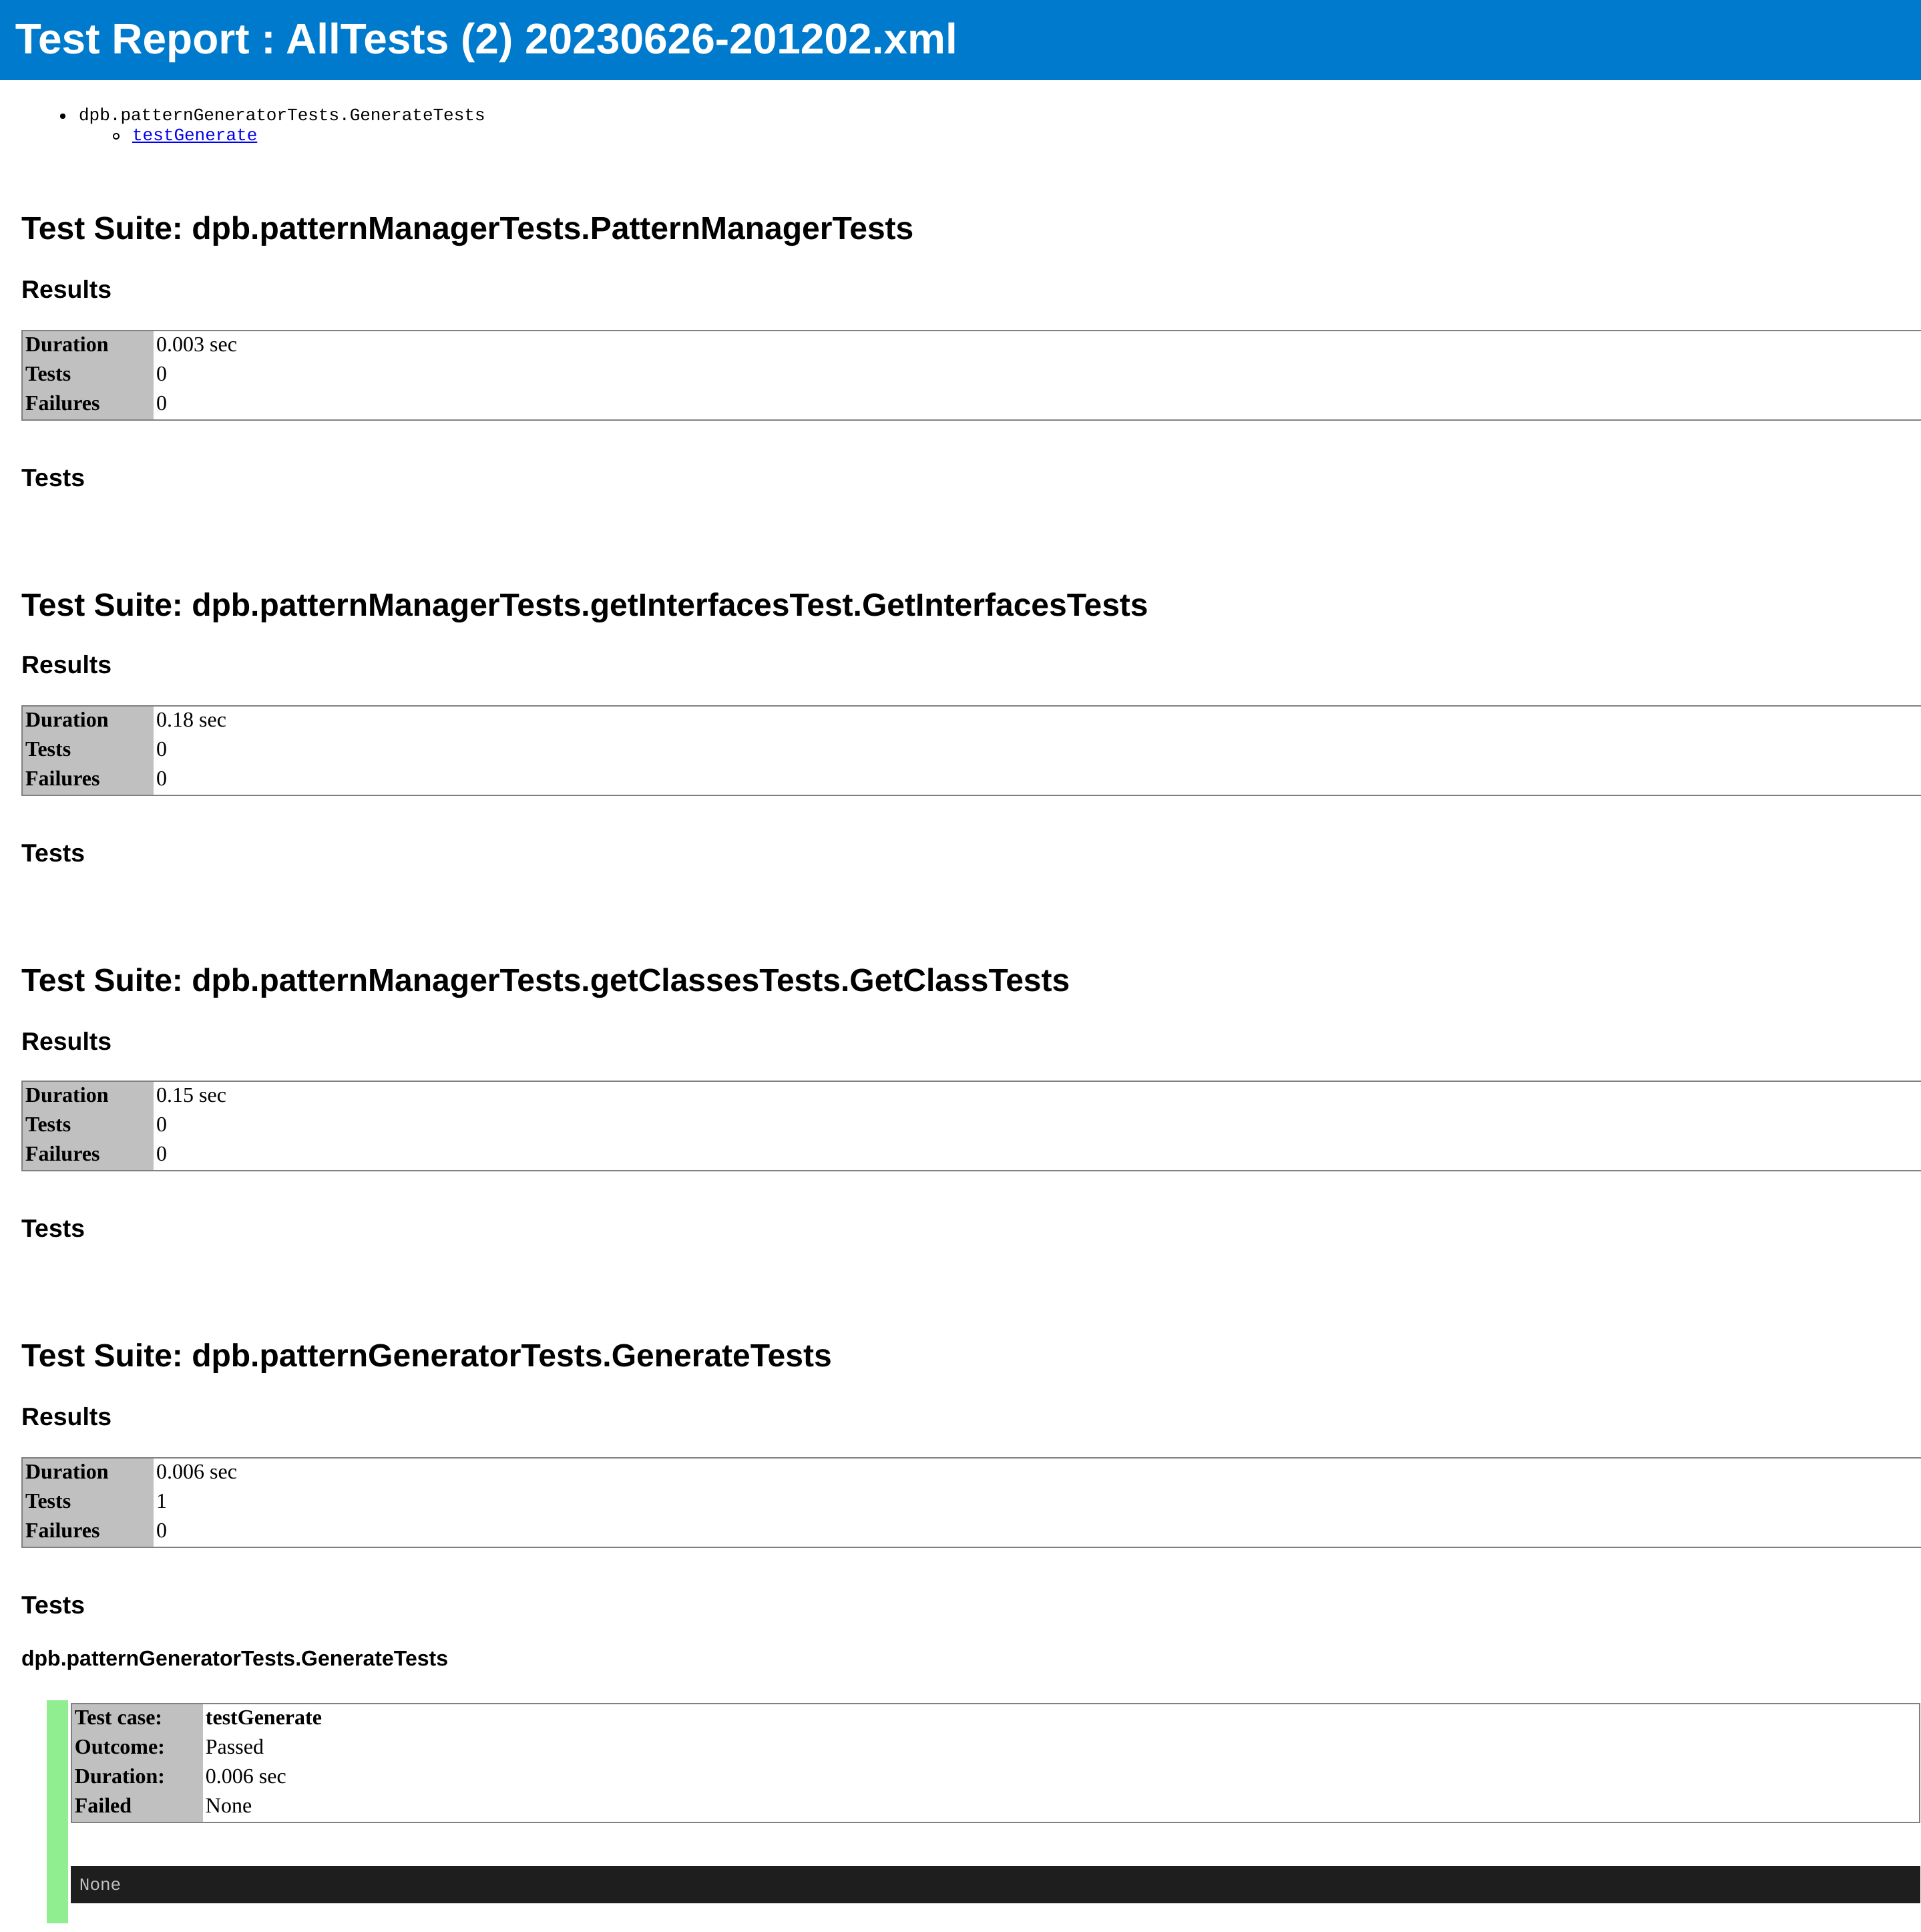
\includegraphics[width=1.0\textwidth]{Figures/test_report.png}
    \label{fig:testReport}
    \caption{Αναφορά αποτελεσμάτων ελέγχων}
\end{figure}